
\section{maincontent}


\begin{frame}
\frametitle{Spin-Polarization Control of Photoelectrons
Using Poincar\'e Fields \\
\small (Extra notes)}
\framesubtitle{Constants}


\footnotesize
\begin{textblock*}{400pt}(30pt,70pt)
\begin{itemize}
\item The normalized field amplitude tells the strength of the field 
relative to the electron rest energy
\begin{align}
a_0 & = \frac{eE}{m_e c\omega}
\end{align}
\item Keldysh parameter tells the regime, tunnel or multiphoton
\begin{equation}
\gamma = \frac{\omega}{E}\sqrt{2m_eI_p} = \sqrt{\frac{2I_p}{m_ea_0^2 c}}
\end{equation}
\item The ionization potential
\begin{equation}
I_p = m_ec^2 -E, \hspace{20pt} \mbox{with} \hspace{20pt}
E = m_e c^2\sqrt{1-(Z\alpha^2)}
\end{equation}
if $Z\alpha \ll 1$, (nonrelativistic case), 
\begin{equation}
I_p \sim \frac{m_eZ\alpha^2c}{2}
\end{equation}
\end{itemize}
\end{textblock*}
 
\end{frame}

\begin{frame}
\frametitle{Spin-Polarization Control of Photoelectrons
Using Poincar\'e Fields \\
\small (Extra notes)}
\framesubtitle{Vector spherical harmonics and the magnetic multipole field}


\footnotesize
\begin{textblock*}{400pt}(30pt,70pt)
\begin{itemize}
\item The multipole order electromagnetic field  is written, 
the poles being magnetic
\begin{align}
\boldsymbol{A}_{jm}(\boldsymbol{k},t) & = 
{\rm Re}\,A_0{\boldsymbol{\Phi}}_{jm}
\left( \theta_{\boldsymbol{k}},\varphi_{\boldsymbol{k}}\right)
\delta(|\boldsymbol{k}|-\omega)e^{i\omega t}, \\
\boldsymbol{A}_{jm}(\boldsymbol{r},t) & = 
{\rm Re}\,A_0 g_j(kr) {\boldsymbol{\Phi}}_{jm}
\left( \theta,\varphi\right) e^{i\omega t},
\end{align}
where ${\boldsymbol{\Phi}}_{jm}
\left( \theta,\varphi\right) =
\hat{\boldsymbol{r}}\times \boldsymbol{\nabla} Y_{jm}
\left( \theta,\varphi\right)$ 
and $g_j(z)=\sqrt{\frac{\pi}{2z}}J_{j+1/2}(z)$ 
is the Bessel function of the first kind
\begin{equation}
%j=\ell+m_s = 1/2 \hspace{40pt}\longrightarrow
%\hspace{40pt}
j\geqslant 1, \hspace{30pt} |m| < j-1 \label{eqn:ineq}
\end{equation}
\input{tables/tab1_supp.tab}

\item $j$ is used not as the sum of $\ell$ and spin $s$, 
but rather as a convention.
\item Notice that the inequality (\ref{eqn:ineq}) is strict
\end{itemize}
\end{textblock*}
 
\end{frame}


\begin{frame}
\frametitle{Spin-Polarization Control of Photoelectrons
Using Poincar\'e Fields \\
\small (Extra notes)}
\framesubtitle{Calculation of helicity}


\footnotesize
\begin{textblock*}{400pt}(30pt,70pt)
\begin{itemize}
\item Using the metric $\left(+,-,-,-\right)$ and having $\boldsymbol{\sigma}$
as the Pauli matrices
\begin{equation}
\gamma^0 \equiv \beta =
\left(
\begin{matrix}
\mathds{1}  & 0          \\
0           & -\mathds{1} 
\end{matrix}\right), \hspace{20pt}
\gamma =
\left(
\begin{matrix}
0                              & \boldsymbol{\sigma}          \\
-\boldsymbol{\sigma}           & 0
\end{matrix}\right), \hspace{20pt}
\alpha = \gamma^0\boldsymbol{\gamma}, \hspace{20pt}
\boldsymbol{\Sigma} =
\left(
\begin{matrix}
\boldsymbol{\sigma}            &        0                    \\
0                              &        \boldsymbol{\sigma}        
\end{matrix}\right).
\end{equation}
\item The helicity of the particle is the projection of its spin along 
$\boldsymbol{n} = \boldsymbol{p}/|\boldsymbol{p}|$ and is 
a "good quantum number"
\item Helicity density is expressed as
\begin{equation}
\zeta(\boldsymbol{p}) = \langle \widetilde{\psi}(\boldsymbol{p}) |
\left( \boldsymbol{n}\cdot\frac{1}{2}\boldsymbol{\Sigma}\right)
|\widetilde{\psi}(\boldsymbol{p})\rangle, \hspace{30pt}
\boldsymbol{n} =
\left(\sin\theta\sin\varphi,\sin\theta\cos\varphi,\cos\varphi\right),
\hspace{20pt}
\end{equation}
\begin{equation}
\zeta(\boldsymbol{p}) = \frac{1}{2}\int d^3\boldsymbol{p}\,
\widetilde{\psi}^{*}(\boldsymbol{p})
\left(\begin{matrix}
\cos\theta               &   \sin\theta e^{-i\varphi} &   0   &    0  \\ 
\sin\theta e^{i\varphi}  & -   \cos\theta             &   0   &    0  \\
0  &   0      & \cos\theta               &   \sin\theta e^{-i\varphi} \\ 
0  &   0      & \sin\theta e^{i\varphi}  & -   \cos\theta             \\
\end{matrix}\right)
\widetilde{\psi}(\boldsymbol{p})
\end{equation}
\vspace{10pt}
\item The case of 
a free electron in its $\gamma=+1/2$ helicity state is in the supp. materials
\end{itemize}
\end{textblock*}



\end{frame}



\begin{frame}
\frametitle{Spin-Polarization Control of Photoelectrons
Using Poincar\'e Fields \\
\small (Extra notes)}
\framesubtitle{Helicity density $\zeta(\boldsymbol{p})$ of ${\rm Ne}^{9+}$ 
- Single mode ionization case -
$(m<0)$}


\begin{textblock*}{200pt}(30pt,60pt)
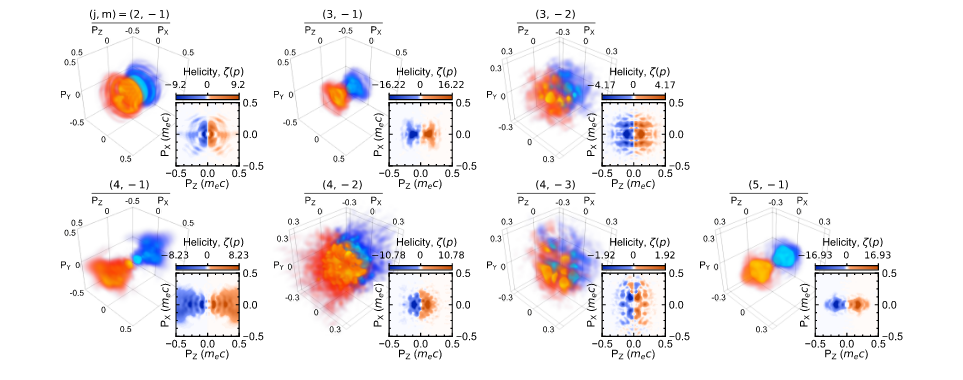
\includegraphics[scale=.33]{images/medium_supp1.png}
\end{textblock*}
%\begin{textblock*}{200pt}(200pt,165pt)
%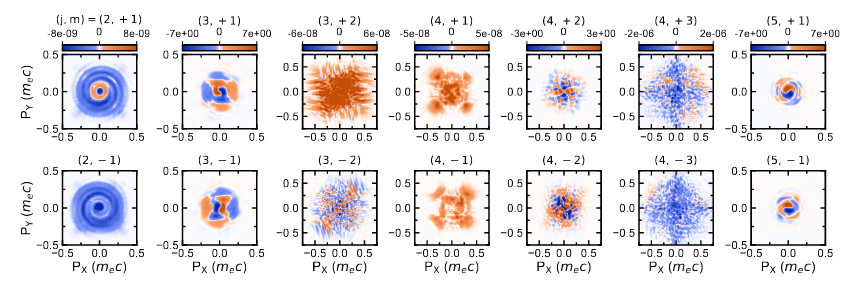
\includegraphics[scale=.28]{images/medium_supp2.png} 
%\end{textblock*}

\end{frame}


\begin{frame}
\frametitle{Spin-Polarization Control of Photoelectrons
Using Poincar\'e Fields \\
\small (Extra notes)}
\framesubtitle{Helicity density $\zeta(\boldsymbol{p})$ of ${\rm Ne}^{9+}$ 
- Single mode ionization case - Integrated}


\begin{textblock*}{200pt}(30pt,60pt)
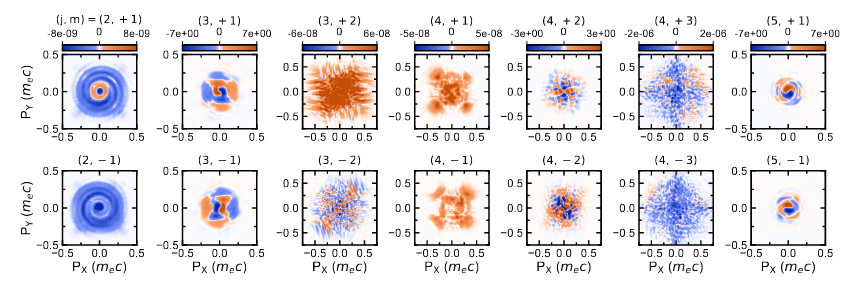
\includegraphics[scale=.33]{images/medium_supp2.png}
\end{textblock*}
\begin{textblock*}{200pt}(130pt,165pt)
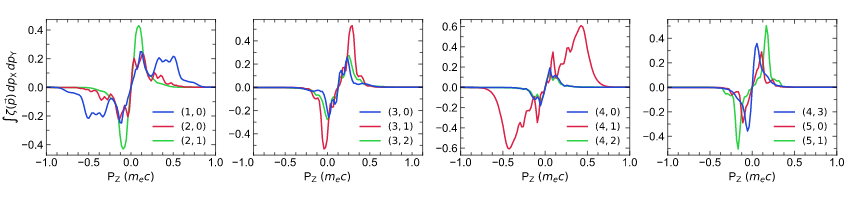
\includegraphics[scale=.36]{images/medium_supp3.png} 
\end{textblock*}



\end{frame}


\begin{frame}
\frametitle{Spin-Polarization Control of Photoelectrons
Using Poincar\'e Fields \\
\small (Extra notes)}
\framesubtitle{Visual effect of the mask function 
$\mathcal{M}_\mu(\boldsymbol{r})$}

\begin{textblock*}{200pt}(30pt,60pt)
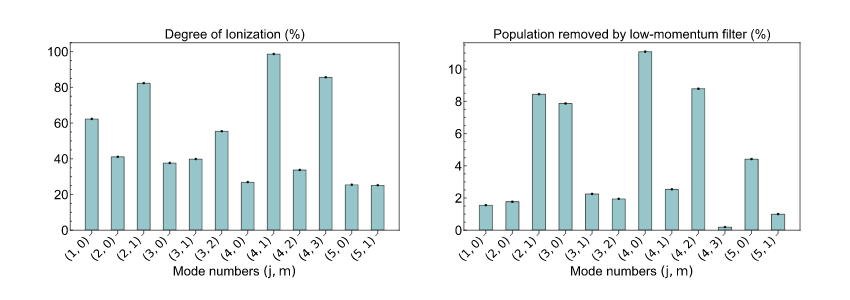
\includegraphics[scale=.33]{images/medium_supp4.png}
\end{textblock*}
\begin{textblock*}{200pt}(160pt,150pt)
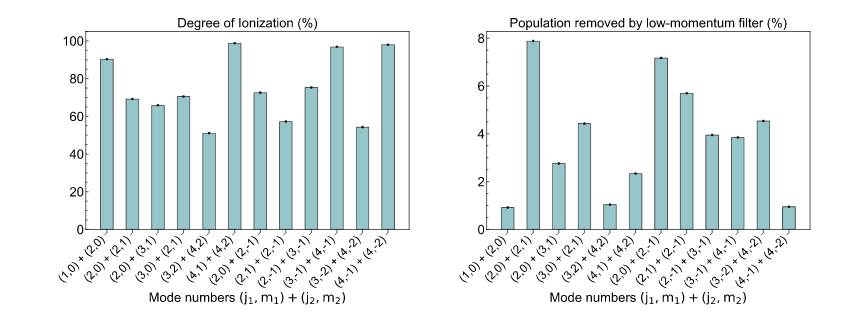
\includegraphics[scale=.33]{images/medium_supp5.png} 
\end{textblock*}

\begin{textblock*}{150pt}(30pt,170pt)
\begin{itemize}
\scriptsize
\item Left : Degree of ionization for each mode, 
bound population was removed by using $\mathcal{M}_\mu(\boldsymbol{r})$
\item Right : Percent of the population removed by the low momentum filter
$\mathcal{M}_\mu(\boldsymbol{p})$
\end{itemize}
\end{textblock*}

\end{frame}







\begin{frame}
\frametitle{Spin-Polarization Control of Photoelectrons
Using Poincar\'e Fields \\
\small (Extra notes)}
\framesubtitle{Helicity density $\zeta(\boldsymbol{p})$ of ${\rm Ar}^{17+}$}


\begin{textblock*}{400pt}(50pt,60pt)
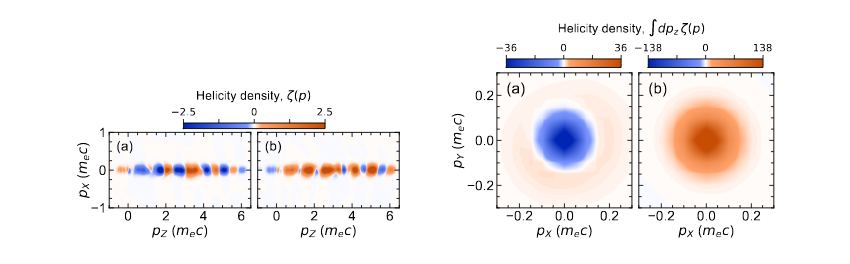
\includegraphics[scale=.40]{images/medium_supp6.png}
\end{textblock*}

\begin{textblock*}{400pt}(30pt,170pt)
\begin{itemize}
\footnotesize
\vspace{10pt}
\item Irradiation by a left-(a) and right-(b) -circularly-polarized field
\item Leftmost panels : Distribution in the $xy$-plane
\item Rightmost panels : Distribution integrated along the $z$ 
momentum direction
\end{itemize}
\vspace{10pt}
\end{textblock*}


\end{frame}
